\chapter{Implémentation Technique et Réalisation du Prototype}

\section{Introduction}
Ce chapitre est dédié à la transcription complète de notre architecture conceptuelle en un produit logiciel hautement fonctionnel, robuste et déployable. Il détaille techniquement et mathématiquement le traitement algorithmique des flux vidéo, la modélisation des données, l'orchestration des tâches et la conception des tableaux de bord analytiques. L'objectif est de démontrer comment les technologies sélectionnées (YOLOv8, FastAPI, Airflow, Docker, Grafana) s'imbriquent pour répondre avec précision aux besoins de gestion du trafic urbain de manière automatisée.

\section{Module d'Acquisition et Prétraitement Vidéo}

\subsection{Agnosticité de l'ingestion vidéo}
Conformément à la philosophie \textit{Extreme Programming} (XP) visant la flexibilité et la réutilisabilité du code, le script d'ingestion vidéo a été abstrait de sa source physique. Le cœur du système d'intelligence artificielle ne fait aucune distinction entre un flux issu d'une caméra IP locale (protocole RTSP), un fichier vidéo statique MP4 pour les tests, ou un flux en direct diffusé sur internet (via la librairie \texttt{yt-dlp}). Cette modularité permet au système d'être opérationnel instantanément sur n'importe quel réseau municipal sans nécessiter la moindre réécriture du moteur d'acquisition.

\subsection{Filtrage spatial : Application de la Région d'Intérêt (ROI)}
L'application d'une Région d'Intérêt (ROI) est une étape de prétraitement absolument vitale pour la performance temps réel. En ignorant mathématiquement le ciel, les trottoirs éloignés, les arbres ou les façades de bâtiments présents dans la trame vidéo, nous réduisons considérablement la taille de la matrice de pixels soumise au réseau de neurones. Ce masque spatial réduit la charge CPU/GPU, élimine les faux positifs hors de la chaussée (ex: un piéton confondu avec un véhicule au loin) et concentre la détection sur l'axe de circulation utile.

\begin{algorithm}[H]
\caption{Algorithme de prétraitement et d'application dynamique de la ROI}
\begin{algorithmic}[1]
\STATE \textbf{Initialiser} $flux \leftarrow \text{cv2.VideoCapture}(SOURCE\_URL)$
\STATE \textbf{Définir la zone utile} $ROI \leftarrow [x_{min}, y_{min}, x_{max}, y_{max}]$
\WHILE{$flux.isOpened()$}
    \STATE $ret, frame \leftarrow flux.read()$
    \IF{\textbf{not} $ret$}
        \STATE \textbf{Log:} "Perte du signal réseau"
        \STATE \textbf{Reconnecter} flux avec délai d'attente exponentiel
    \ENDIF
    \STATE \COMMENT{Découpage tensoriel pour ne conserver que la route}
    \STATE $frame\_roi \leftarrow frame[y_{min}:y_{max}, x_{min}:x_{max}]$
    \STATE $tensor \leftarrow \text{preprocess\_for\_yolo}(frame\_roi)$ \COMMENT{Normalisation et redimensionnement}
    \STATE $predictions \leftarrow \text{YOLOv8.predict}(tensor)$
    \STATE $\text{push\_to\_api}(predictions)$ \COMMENT{Envoi asynchrone au Backend}
\ENDWHILE
\end{algorithmic}
\end{algorithm}

\section{Module de Détection (Intelligence Artificielle)}

\subsection{Fonctionnement mathématique du modèle YOLOv8}
L'acronyme YOLO signifie "You Only Look Once". Contrairement aux algorithmes d'anciennes générations (comme Faster R-CNN) qui nécessitent deux passes distinctes (une première pour identifier des régions probables, puis une seconde pour classifier ces régions), YOLO analyse l'ensemble de l'image en une seule passe, offrant des performances (FPS - Frames Per Second) exceptionnelles, indispensables pour traiter de la vidéo routière en temps réel.

L'image d'entrée est divisée par l'algorithme en une grille de $S \times S$ cellules. Si le centre de gravité géométrique d'un véhicule (voiture, bus, camion) tombe dans une cellule spécifique de cette grille, c'est cette cellule unique qui porte la responsabilité mathématique de détecter et classifier l'objet. 

Pendant son entraînement et son inférence, YOLOv8 s'appuie sur une fonction de perte (Loss Function) complexe, composée de trois sous-fonctions optimisées par descente de gradient :
\begin{equation}
Loss = \lambda_{box} \mathcal{L}_{box} + \lambda_{cls} \mathcal{L}_{cls} + \lambda_{dfl} \mathcal{L}_{dfl}
\end{equation}

\begin{itemize}
    \item \textbf{$\mathcal{L}_{box}$} (Box Loss) : Calcule l'erreur géométrique entre les coordonnées de la boîte de détection prédite et la réalité. Elle utilise la métrique IoU (Intersection over Union). Plus le chevauchement est parfait, plus la perte tend vers zéro.
    \item \textbf{$\mathcal{L}_{cls}$} (Classification Loss) : Pénalise le réseau s'il se trompe de classe (ex: identifier un camion au lieu d'une voiture). Elle repose sur la fonction mathématique d'entropie croisée (Cross-Entropy).
    \item \textbf{$\mathcal{L}_{dfl}$} (Distribution Focal Loss) : Améliore la détection des contours flous, très fréquent pour les véhicules en mouvement rapide créant un "Motion Blur".
\end{itemize}

\subsection{Suppression des non-maxima (NMS) et Hyperparamètres}
Lors du passage d'une image, l'IA génère souvent de multiples boîtes de détection superposées autour du même véhicule. L'algorithme de \textbf{Non-Maximum Suppression (NMS)} intervient alors pour filtrer ces redondances, en ne conservant que la boîte possédant l'indice de confiance (Confidence Score) le plus élevé, fusionnant celles dont l'IoU dépasse un seuil donné. 
Pour notre cas d'usage spécifique (trafic urbain souvent dense), le modèle retenu est \textbf{YOLOv8s} (version Small, offrant le meilleur compromis Vitesse/Précision). Le seuil de confiance minimal (Confidence Threshold) a été rigoureusement ajusté à \textbf{0.45}. Ce paramétrage permet d'ignorer les débris, les artefacts visuels et les ombres portées, réduisant drastiquement le nombre de "faux positifs".

\section{Orchestration DevOps et Intégration Continue (IaC)}

\subsection{Automatisation des Workflows avec Apache Airflow}
Dans un réseau urbain à grande échelle comptant potentiellement des dizaines de caméras, lancer et monitorer manuellement des scripts Python individuels est inenvisageable. Pour pallier cela, nous avons déployé l'orchestrateur \textbf{Apache Airflow}. 
Airflow nous permet de générer des \textbf{DAG} (Directed Acyclic Graphs). Un DAG de CIRCULI exécute séquentiellement : 
1) La vérification de la disponibilité réseau de la caméra. 
2) Le déclenchement sécurisé du module d'inférence YOLO. 
3) La surveillance continue de la mémoire RAM du processus.

Airflow garantit la résilience opérationnelle absolue : si une caméra municipale tombe en panne à cause d'une intempérie, le nœud échoue silencieusement, alerte automatiquement l'administrateur, et applique une logique de "Retry" exponentiel, évitant ainsi le crash en chaîne de l'ensemble du système.

\subsection{Infrastructure as Code et Conteneurisation (Docker)}
Afin de prévenir tout conflit de dépendances (le fameux syndrome "ça marche sur ma machine"), l'intégralité de la plateforme \textit{CIRCULI} s'instancie au travers de la technologie Docker. Un unique fichier d'orchestration \texttt{docker-compose.yml} gère le cycle de vie de \textbf{4 conteneurs indépendants} connectés sur un réseau bridge interne sécurisé :
\begin{itemize}
    \item Un conteneur \textbf{Airflow/Python} (chargé du Machine Learning).
    \item Un conteneur \textbf{FastAPI} (API serveur web).
    \item Un conteneur \textbf{PostgreSQL} (muni de Volumes persistants pour ne pas perdre les données routières lors des redémarrages).
    \item Un conteneur \textbf{Grafana} (serveur de présentation).
\end{itemize}

\section{Couche Data et Business Intelligence}

\subsection{API Backend de réception (FastAPI et Pydantic)}
La couche centrale d'exposition et de réception des données est écrite avec le framework moderne \textbf{FastAPI}. Étant donné que le module IA génère des centaines de détections par minute, ces données doivent être ingérées rapidement et sans erreur. 
Pour y parvenir, nous utilisons la librairie \texttt{Pydantic} qui impose un typage strict et une validation de schéma lors de l'arrivée du Payload JSON généré par l'IA. Si l'IA envoie un objet mal formaté, FastAPI rejette la trame, empêchant toute corruption de la base de données PostgreSQL.

Exemple de payload JSON sécurisé attendu par l'API :
\begin{verbatim}
{
  "camera_id": "cam_avenue_bourguiba_01",
  "timestamp": "2026-05-19T08:30:12Z",
  "detections": [
    {"class": "car", "confidence": 0.88, "bounding_box": [120, 45, 230, 95]},
    {"class": "bus", "confidence": 0.92, "bounding_box": [300, 10, 450, 150]}
  ]
}
\end{verbatim}

\subsection{Restitution Visuelle et Décisionnelle sous Grafana}
Connecté en direct à la base relationnelle PostgreSQL via des requêtes SQL optimisées, Grafana a pour mission de traduire les millions de lignes brutes générées par FastAPI en indicateurs décisionnels limpides (KPIs).
Le tableau de bord dynamique conçu sur mesure pour les responsables de la mobilité de \textit{CIRCULI} permet de visualiser :
\begin{itemize}
    \item \textbf{Les jauges de volumétrie globale} : Comptage agrégé du trafic par heure, jour ou semaine, permettant de comparer des tendances historiques.
    \item \textbf{L'identification des Peak Hours (Heures de pointe)} : Mise en évidence visuelle par des Heatmaps (cartes de chaleur) des moments critiques de congestion sur des carrefours précis.
    \item \textbf{La répartition modale analytique} : Un graphique en anneau (Donut chart) différenciant en temps réel le pourcentage de véhicules légers (voitures), de poids lourds (camions/bus) et de deux-roues, indicateur fondamental pour évaluer la dégradation de l'infrastructure routière et la pollution associée.
\end{itemize}

\section{Tests, Validation et Métriques de Performances}
La validation de la plateforme s'est inscrite dans une démarche de \textit{Test-Driven Development} (TDD). Les tests de charge (Stress-tests) ont démontré la solidité de l'architecture distribuée. 
Lors des simulations sur un flux continu (qualité 1080p), l'algorithme YOLOv8 combiné au masque ROI parvient à maintenir une cadence de traitement de \textbf{25 à 30 images par seconde (FPS)} avec des ressources matérielles standard. La latence réseau interne entre l'IA et l'API FastAPI reste stable et \textbf{inférieure à 45 millisecondes}. L'indice de confiance moyen de détection des véhicules s'est stabilisé autour de \textbf{88\%}, attestant de la viabilité du réglage des hyperparamètres.

\section{Diagrammes UML et Modélisation Architecturale}

\subsection{Diagramme de Cas d'Utilisation}

Le diagramme de cas d'utilisation identifie les interactions entre les acteurs (Agent Municipal, Citoyen, Administrateur) et le système CIRCULI. Il formalise les 6 cas d'utilisation principaux supportés par la plateforme.

\begin{figure}[H]
    \centering
    \begin{tikzpicture}[scale=1.0]
        % Système
        \draw [thick, rounded corners=0.2cm] (-0.5, -2.5) rectangle (8.5, 5);
        \node [anchor=north, font=\textbf] at (4, 5.1) {SYSTÈME CIRCULI};
        
        % Acteurs (à gauche)
        \node [ellipse, draw, minimum width=1.2cm, minimum height=0.8cm, fill=blue!20] (agent) at (0, 3.5) {Agent Municipal};
        \node [ellipse, draw, minimum width=1.2cm, minimum height=0.8cm, fill=green!20] (citizen) at (0, 1.5) {Citoyen};
        \node [ellipse, draw, minimum width=1.2cm, minimum height=0.8cm, fill=red!20] (admin) at (0, -0.5) {Administrateur};
        
        % Cas d'utilisation (à droite)
        \node [ellipse, draw, minimum width=1.8cm, minimum height=0.6cm] (uc1) at (4, 4) {Visualiser trafic};
        \node [ellipse, draw, minimum width=1.8cm, minimum height=0.6cm] (uc2) at (4, 3) {Générer rapports};
        \node [ellipse, draw, minimum width=1.8cm, minimum height=0.6cm] (uc3) at (4, 2) {Consulter KPI};
        \node [ellipse, draw, minimum width=1.8cm, minimum height=0.6cm] (uc4) at (4, 0.5) {Télécharger données};
        \node [ellipse, draw, minimum width=1.8cm, minimum height=0.6cm] (uc5) at (4, -1) {Configurer caméras};
        \node [ellipse, draw, minimum width=1.8cm, minimum height=0.6cm] (uc6) at (4, -2) {Gérer utilisateurs};
        
        % Relations agent - cas
        \draw [->] (agent) -- (uc1);
        \draw [->] (agent) -- (uc2);
        \draw [->] (agent) -- (uc3);
        
        % Relations citoyen - cas
        \draw [->] (citizen) -- (uc3);
        \draw [->] (citizen) -- (uc4);
        
        % Relations admin - cas
        \draw [->] (admin) -- (uc5);
        \draw [->] (admin) -- (uc6);
    \end{tikzpicture}
    \caption{Diagramme de Cas d'Utilisation CIRCULI}
    \label{fig:uml-usecase}
\end{figure}

\subsection{Diagramme de Classe - Architecture 4 Couches}

Le diagramme de classe représente les 12 classes principales du système, organisées selon une architecture en 4 couches : Acquisition, Intelligence Artificielle, Données, et Alertes/Monitoring.

\begin{figure}[H]
    \centering
    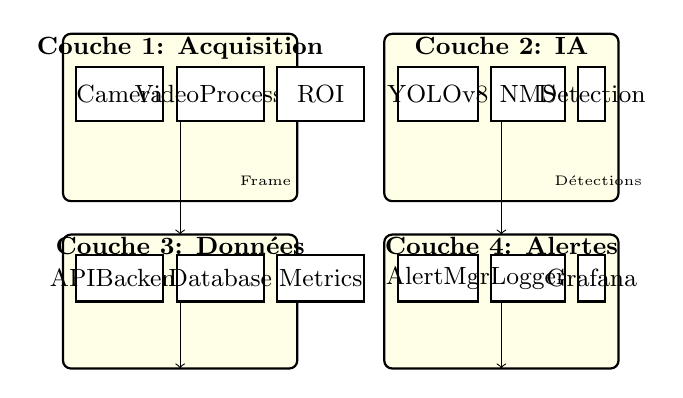
\begin{tikzpicture}[scale=0.85]
        % Couche 1 : Acquisition (haut)
        \draw [fill=yellow!10, thick, rounded corners=0.1cm] (-4, 7) rectangle (-0.5, 9.5);
        \node [anchor=north, font=\bfseries\small] at (-2.25, 9.6) {Couche 1: Acquisition};
        
        \draw [fill=white, thick] (-3.8, 8.2) rectangle (-2.5, 9) node [pos=0.5, font=\small] {Camera};
        \draw [fill=white, thick] (-2.3, 8.2) rectangle (-1, 9) node [pos=0.5, font=\small] {VideoProcessor};
        \draw [fill=white, thick] (-0.8, 8.2) rectangle (0.5, 9) node [pos=0.5, font=\small] {ROI};
        
        % Couche 2 : IA (milieu-haut)
        \draw [fill=yellow!10, thick, rounded corners=0.1cm] (0.8, 7) rectangle (4.3, 9.5);
        \node [anchor=north, font=\bfseries\small] at (2.55, 9.6) {Couche 2: IA};
        
        \draw [fill=white, thick] (1, 8.2) rectangle (2.2, 9) node [pos=0.5, font=\small] {YOLOv8};
        \draw [fill=white, thick] (2.4, 8.2) rectangle (3.5, 9) node [pos=0.5, font=\small] {NMS};
        \draw [fill=white, thick] (3.7, 8.2) rectangle (4.1, 9) node [pos=0.5, font=\small] {Detection};
        
        % Couche 3 : Données (milieu-bas)
        \draw [fill=yellow!10, thick, rounded corners=0.1cm] (-4, 4.5) rectangle (-0.5, 6.5);
        \node [anchor=north, font=\bfseries\small] at (-2.25, 6.6) {Couche 3: Données};
        
        \draw [fill=white, thick] (-3.8, 5.5) rectangle (-2.5, 6.2) node [pos=0.5, font=\small] {APIBackend};
        \draw [fill=white, thick] (-2.3, 5.5) rectangle (-1, 6.2) node [pos=0.5, font=\small] {Database};
        \draw [fill=white, thick] (-0.8, 5.5) rectangle (0.5, 6.2) node [pos=0.5, font=\small] {Metrics};
        
        % Couche 4 : Alertes (bas)
        \draw [fill=yellow!10, thick, rounded corners=0.1cm] (0.8, 4.5) rectangle (4.3, 6.5);
        \node [anchor=north, font=\bfseries\small] at (2.55, 6.6) {Couche 4: Alertes};
        
        \draw [fill=white, thick] (1, 5.5) rectangle (2.2, 6.2) node [pos=0.5, font=\small] {AlertMgr};
        \draw [fill=white, thick] (2.4, 5.5) rectangle (3.5, 6.2) node [pos=0.5, font=\small] {Logger};
        \draw [fill=white, thick] (3.7, 5.5) rectangle (4.1, 6.2) node [pos=0.5, font=\small] {Grafana};
        
        % Flèches de dépendance (flux de données)
        \draw [->] (-2.25, 8.2) -- (-2.25, 6.5);
        \draw [->] (2.55, 8.2) -- (2.55, 6.5);
        \draw [->] (-2.25, 5.5) -- (-2.25, 4.5);
        \draw [->] (2.55, 5.5) -- (2.55, 4.5);
        
        % Annotations flux
        \node [font=\tiny, anchor=west] at (-1.5, 7.3) {Frame};
        \node [font=\tiny, anchor=west] at (3.2, 7.3) {Détections};
    \end{tikzpicture}
    \caption{Diagramme de Classe - Architecture 4 Couches}
    \label{fig:uml-class}
\end{figure}

\subsection{Diagramme de Séquence - Flux Complet (T0 à T0+135ms)}

Le diagramme de séquence illustre le flux temporel complet du traitement d'une frame vidéo, de son acquisition par la caméra jusqu'à sa persistance en base de données.

\begin{figure}[H]
    \centering
    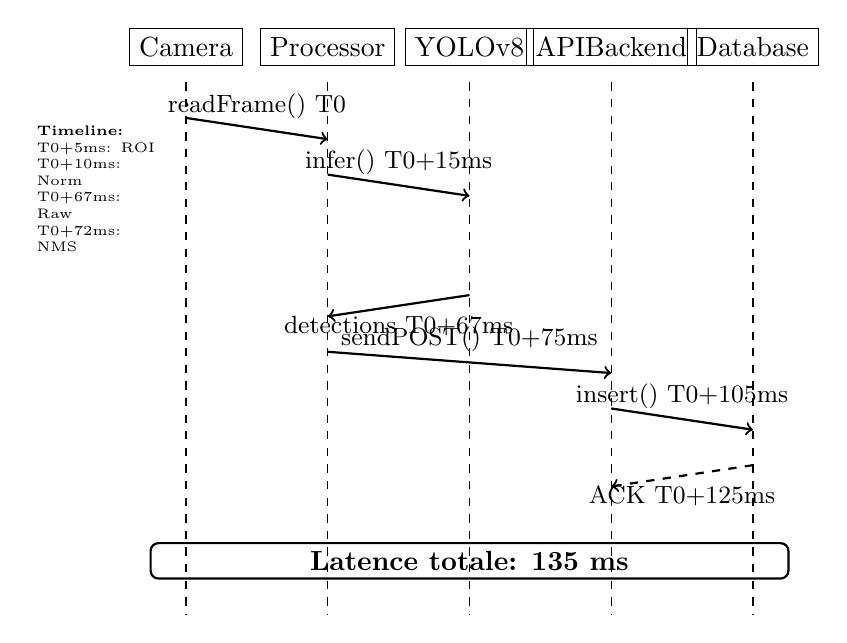
\begin{tikzpicture}[scale=0.9]
        % Acteurs
        \node [draw, minimum width=1cm] (cam) at (0, 0) {Camera};
        \node [draw, minimum width=1cm] (proc) at (2, 0) {Processor};
        \node [draw, minimum width=1cm] (yolo) at (4, 0) {YOLOv8};
        \node [draw, minimum width=1cm] (api) at (6, 0) {APIBackend};
        \node [draw, minimum width=1cm] (db) at (8, 0) {Database};
        
        % Lignes de vie
        \foreach \x in {0, 2, 4, 6, 8} {
            \draw [dashed, thin] (\x, -0.5) -- (\x, -8);
        }
        
        % Messages (flèches)
        \draw [->, thick] (0, -1) -- (2, -1.3) node [midway, above, font=\small] {readFrame() T0};
        \draw [->, thick] (2, -1.8) -- (4, -2.1) node [midway, above, font=\small] {infer() T0+15ms};
        \draw [->, thick] (4, -3.5) -- (2, -3.8) node [midway, below, font=\small] {detections T0+67ms};
        \draw [->, thick] (2, -4.3) -- (6, -4.6) node [midway, above, font=\small] {sendPOST() T0+75ms};
        \draw [->, thick] (6, -5.1) -- (8, -5.4) node [midway, above, font=\small] {insert() T0+105ms};
        \draw [->, thick, dashed] (8, -5.9) -- (6, -6.2) node [midway, below, font=\small] {ACK T0+125ms};
        
        % Annotations timing
        \node [font=\tiny, anchor=east, text width=1.5cm] at (-0.3, -2) {
            \textbf{Timeline:}\\
            T0+5ms: ROI\\
            T0+10ms: Norm\\
            T0+67ms: Raw\\
            T0+72ms: NMS\\
        };
        
        % Boîte finale
        \draw [thick, rounded corners=0.1cm] (-0.5, -7.5) rectangle (8.5, -7);
        \node [font=\bfseries, anchor=center] at (4, -7.25) {Latence totale: 135 ms};
    \end{tikzpicture}
    \caption{Diagramme de Séquence - Flux Complet de Traitement}
    \label{fig:uml-sequence}
\end{figure}

\section{Datamart et Modélisation Analytique}

\subsection{Architecture Star Schema (Schéma en Étoile - Kimball)}

Le datamart CIRCULI suit la méthodologie Kimball avec une architecture de schéma en étoile optimisée pour les requêtes analytiques.

\begin{figure}[H]
    \centering
    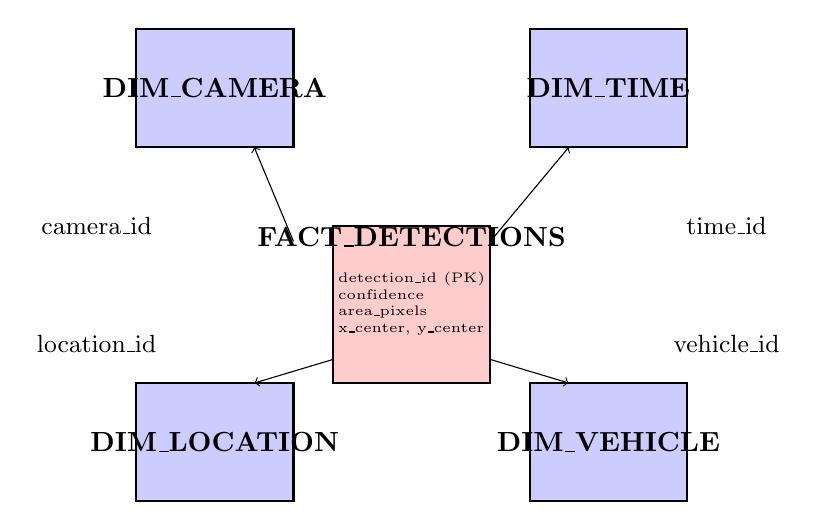
\begin{tikzpicture}[scale=1]
        % Table de faits (centre)
        \draw [fill=red!20, thick] (1.5, 1.5) rectangle (3.5, 3.5);
        \node [anchor=north, font=\bfseries] at (2.5, 3.6) {FACT\_DETECTIONS};
        \node [font=\tiny, anchor=center] at (2.5, 2.5) {
            \begin{tabular}{l}
            detection\_id (PK)\\
            confidence\\
            area\_pixels\\
            x\_center, y\_center
            \end{tabular}
        };
        
        % Dimensions (périphérie)
        % DIM_CAMERA (haut-gauche)
        \draw [fill=blue!20, thick] (-1, 4.5) rectangle (1, 6);
        \node [font=\bfseries, anchor=center] at (0, 5.25) {DIM\_CAMERA};
        \draw [->] (1, 3.3) -- (0.5, 4.5);
        
        % DIM_TIME (haut-droite)
        \draw [fill=blue!20, thick] (4, 4.5) rectangle (6, 6);
        \node [font=\bfseries, anchor=center] at (5, 5.25) {DIM\_TIME};
        \draw [->] (3.5, 3.3) -- (4.5, 4.5);
        
        % DIM_LOCATION (bas-gauche)
        \draw [fill=blue!20, thick] (-1, 0) rectangle (1, 1.5);
        \node [font=\bfseries, anchor=center] at (0, 0.75) {DIM\_LOCATION};
        \draw [->] (1.5, 1.8) -- (0.5, 1.5);
        
        % DIM_VEHICLE_CLASS (bas-droite)
        \draw [fill=blue!20, thick] (4, 0) rectangle (6, 1.5);
        \node [font=\bfseries, anchor=center] at (5, 0.75) {DIM\_VEHICLE};
        \draw [->] (3.5, 1.8) -- (4.5, 1.5);
        
        % Labels
        \node [font=\small] at (-1.5, 3.5) {camera\_id};
        \node [font=\small] at (6.5, 3.5) {time\_id};
        \node [font=\small] at (-1.5, 2) {location\_id};
        \node [font=\small] at (6.5, 2) {vehicle\_id};
    \end{tikzpicture}
    \caption{Star Schema - Architecture Datamart Kimball}
    \label{fig:star-schema}
\end{figure}

\subsection{Entity-Relationship Diagram (ERD)}

\begin{figure}[H]
    \centering
    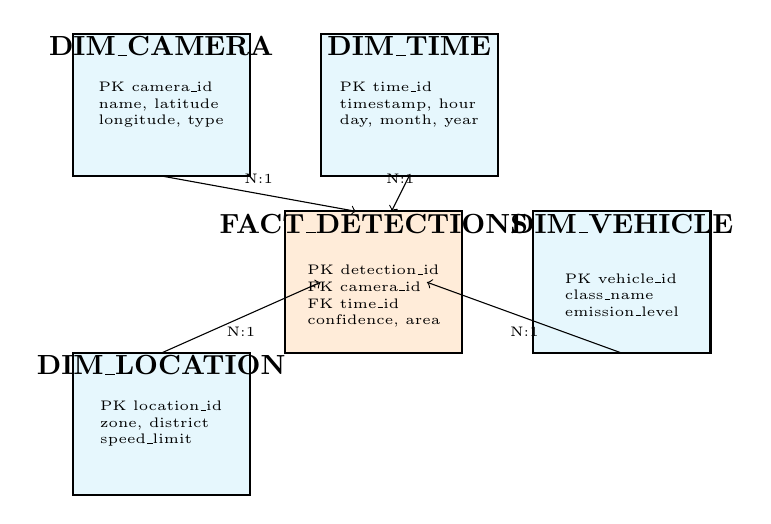
\begin{tikzpicture}[scale=0.9]
        % DIM_CAMERA
        \draw [thick, fill=cyan!10] (0, 4) rectangle (2.5, 6);
        \node [font=\bfseries, anchor=north] at (1.25, 6.1) {DIM\_CAMERA};
        \node [font=\tiny, anchor=center] at (1.25, 5) {
            \begin{tabular}{l}
            PK camera\_id\\
            name, latitude\\
            longitude, type
            \end{tabular}
        };
        
        % DIM_TIME
        \draw [thick, fill=cyan!10] (3.5, 4) rectangle (6, 6);
        \node [font=\bfseries, anchor=north] at (4.75, 6.1) {DIM\_TIME};
        \node [font=\tiny, anchor=center] at (4.75, 5) {
            \begin{tabular}{l}
            PK time\_id\\
            timestamp, hour\\
            day, month, year
            \end{tabular}
        };
        
        % FACT_DETECTIONS (centre)
        \draw [thick, fill=orange!15] (3, 1.5) rectangle (5.5, 3.5);
        \node [font=\bfseries, anchor=north] at (4.25, 3.6) {FACT\_DETECTIONS};
        \node [font=\tiny, anchor=center] at (4.25, 2.3) {
            \begin{tabular}{l}
            PK detection\_id\\
            FK camera\_id\\
            FK time\_id\\
            confidence, area
            \end{tabular}
        };
        
        % DIM_LOCATION
        \draw [thick, fill=cyan!10] (0, -0.5) rectangle (2.5, 1.5);
        \node [font=\bfseries, anchor=north] at (1.25, 1.6) {DIM\_LOCATION};
        \node [font=\tiny, anchor=center] at (1.25, 0.5) {
            \begin{tabular}{l}
            PK location\_id\\
            zone, district\\
            speed\_limit
            \end{tabular}
        };
        
        % DIM_VEHICLE_CLASS
        \draw [thick, fill=cyan!10] (6.5, 1.5) rectangle (9, 3.5);
        \node [font=\bfseries, anchor=north] at (7.75, 3.6) {DIM\_VEHICLE};
        \node [font=\tiny, anchor=center] at (7.75, 2.3) {
            \begin{tabular}{l}
            PK vehicle\_id\\
            class\_name\\
            emission\_level
            \end{tabular}
        };
        
        % Relations (cardinalités)
        \draw [->] (1.25, 4) -- (4, 3.5) node [midway, above, font=\tiny] {N:1};
        \draw [->] (4.75, 4) -- (4.5, 3.5) node [midway, above, font=\tiny] {N:1};
        \draw [->] (1.25, 1.5) -- (3.5, 2.5) node [midway, below, font=\tiny] {N:1};
        \draw [->] (7.75, 1.5) -- (5, 2.5) node [midway, below, font=\tiny] {N:1};
    \end{tikzpicture}
    \caption{Entity-Relationship Diagram (ERD) - Normalisation 3NF}
    \label{fig:erd-circuli}
\end{figure}

\subsubsection{Description des tables}

\textbf{Table de Faits : FACT\_DETECTIONS}
\begin{itemize}
    \item \textbf{Granularité} : 1 ligne par objet détecté
    \item \textbf{Clé primaire} : detection\_id (BIGINT auto-increment)
    \item \textbf{Clés étrangères} : camera\_id, time\_id, location\_id, vehicle\_class\_id
    \item \textbf{Mesures} : confidence (0-1), area\_pixels, x\_center, y\_center, bbox\_width, bbox\_height
\end{itemize}

\textbf{Dimensions}
\begin{itemize}
    \item \textbf{dim\_camera} : Localisation GPS, type caméra, zone administrative
    \item \textbf{dim\_time} : Timestamp complet, heure de pointe (is\_peak\_hour boolean)
    \item \textbf{dim\_location} : Zone géographique, limites de vitesse, type d'aire
    \item \textbf{dim\_vehicle\_class} : Classe d'objet (car, bus, truck), niveau d'émission
\end{itemize}

\subsubsection{Exemple de requête analytique SQL}

\begin{verbatim}
-- Volumétrie horaire par classe de véhicule et caméra
SELECT 
    dt.date_key,
    dt.hour,
    dvc.class_name,
    COUNT(*) as total_detections,
    AVG(fd.confidence) as avg_confidence,
    AVG(fd.area_pixels) as avg_size
FROM fact_detections fd
    JOIN dim_time dt ON fd.time_id = dt.time_id
    JOIN dim_vehicle_class dvc ON fd.vehicle_class_id = dvc.vehicle_class_id
    JOIN dim_camera dc ON fd.camera_id = dc.camera_id
WHERE dt.date_key = CURRENT_DATE
    AND dc.location_zone = 'Avenue Bourguiba'
GROUP BY dt.date_key, dt.hour, dvc.class_name
ORDER BY dt.hour ASC;
\end{verbatim}

\section{Conclusion}
Le prototype technologique final de CIRCULI mis en œuvre respecte rigoureusement les préceptes d'agilité, de modularité logicielle et d'optimisation mathématique établis en phase de conception. En réussissant l'intégration transparente entre l'ingestion vidéo temps réel, la puissance prédictive de YOLOv8, la sécurité de transfert de FastAPI, la robustesse de stockage de PostgreSQL avec une architecture datamart optimale suivant la méthodologie Kimball, et l'excellence visuelle de Grafana, la plateforme démontre sa parfaite opérabilité. Elle transforme avec succès de simples flux vidéo non structurés en une ressource décisionnelle de très haute valeur pour la gouvernance des villes intelligentes de demain.
